\section{Experiment 1}
	
	\textbf{Research Question:} When do unrelated Acoustic Classification tasks, learned in a deep learning multi-task, hard parameter sharing set-up, improve each other? \\
	\textbf{Research Method:} Implement different multi-class acoustic classification tasks from different corpi and different domains. The classification model will be a DNN without any adjustments for any specific task, to generalize the observations for task interaction in a multi-task learning setting. Different measurements are taken from the datasets beforehand. Each task is run in a single task set up, with different measurements being kept from the learning process and results. The goal of the investigation is to assess whether improved performance for one of the tasks in a dual task learning set-up can be achieved, or to which degree these tasks can be combined without a significant performance decrease for efficiency purposes.\\
	
	\textbf{Task choice:}\\
	
	Main Tasks\\
	
%	-- EXPLANATIONS OF TASKS\\
	\begin{itemize}
		\item General Acoustic Event Detection: Acoustic event detection or Sound event detection refers to the task of locating and classifying Sound Events in an audio from real life environments. General purpose AED means no specific optim
		\item Acoustic Scene Classification: Acoustic Scene Classification involves the automatic detection of the environment in an audio stream. Both indoor as well as outdoor environments can be included, with the length duration of a scene being long.
		\item Speaker Identification is the task of identifying the person speaking in an audio clip.
		\item Keyword Spotting aims at detecting predefined keywords in audio streams.
	\end{itemize}

%	-- REASONS WHY FOR THESE TASKS (use in other and general interest)\\
%	- Georgiev used them\\
%	- Most interesting for lifelogging purposes according to gurrin\\
%	- Different and multiple domains\\
%	- Domains: Speech, Environment, Music\\
%	- Different and multiple corpuses\\

	
	These are the main tasks, chosen to represent a variety of audio sensing tasks in the research. The tasks are more often then not the primary focus in audio sensing research, and are more complex in nature, with a multi-class classification goal. The choice was made for this specific set of tasks for multiple reasons. First of all, Gurrin et al. identified the main interests for audio sensing tasks for lifelogging purposes as being the identification of activities, audio events, location, people and keywords in dialogue, each of which is represented as a main task here. Futhermore, in work done by Georgiev, a system is built which combined Acoustic Scene Classification, Speaker Identification, Emotion Recognition and Stress detection, finding that all could be combined in a single multi-task DNN set-up without significant performance decrease. In this work the same DNN structure will as it has shown to perform well on multiple audio sensing tasks as well as allow direct verification for its findings. Furthermore are all (main and auxiliary) tasks chosen so that they would span multiple domains (Speech, Environment and Music), as well as multiple different datasets. \\

	
	\textbf{Neural Network:}\\
	%-- REFER TO GEORGIEV'S USE AND NLP RESEARCH JUSTIFICATION FOR USING 1\\
	
	\begin{figure}
		\centering
		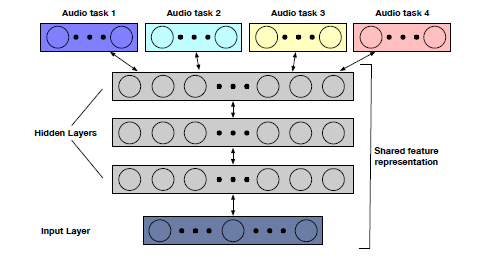
\includegraphics[width=0.9\linewidth]{NN.PNG}
		\caption{Multi-task DNN model}
		\label{fig:NN}
	\end{figure}

	%Basis: DNN feed-forward propagation classifier
	%Input: Statistical summaries of log filter banks
	%Architecture: Input and hidden layers are shared across potential combinations of audio analysis tasks -> Universal feature transformation that captures acoustic observations. 3 hidden layers with either 128, 256 or 512 nodes each, hard parameter sharing. Soft-max layer at the task-specific layers, updated separately depending on the training input instance.
	%Training: mini-batch stochastic gradient descent all audio tasks simultaneously
	%Fine-tuning: backpropagation
	%Additional: Keep the hyper-parameters fixed across single-task and multi-task settings for comparison. Use fixed random seed set upfront to facilitate replicability. Do not use any task-specific features or pre-trained embeddings for initialisation to delimit the behaviour of the architecture and analyse the interaction between tasks.
	
	The architecture is based on the system, described by \citet{georgiev2017heterogeneous}, which is a Deep Neural Network (DNN) feed-forward propagation classifier. As seen in figure \ref{fig:NN}, in a multi-task setting, all tasks share the same input and hidden layers, with task-specific output layers. This leads to these layers being used as a universal feature transformation which captures acoustic observations from different tasks. For the input, features have to be extracted from the audio. In the original work this is implemented by statistical summaries of log filter banks, extracted from each audio frame. They use summaries both for reducing the input feature complexity as well as allowing a representation of the same size across multiple tasks. \\
	
	To allow for comparison and analysis of the interaction between tasks, this work follows the approach from \cite{alonso2016multitask} and \cite{bingel2017identifying} the hyperparameters (this includes a fixed random seed set) and the architecture will be kept the same, regardless of which and the number of tasks learned. The set-up \citet{georgiev2017heterogeneous} had was 3 hidden layers which were tested at 128, 256 or 512 in each layer, with a soft-max pooling layer at the output layers. The output layers are updated separately depending on whether the training input instance is one for their own task. Furthermore, no task-specific features, nor any pre-trained embeddings will be used for initialisation to avoid any task bias. \\
	
	The training is done by mini-batch Stochastic Gradient Descent (SGD) on all audio tasks simultaneously, which is the key to succesfully training the multi-task DNN \citep{georgiev2017heterogeneous}. The samples are randomised across tasks before being fed into the DNN system. Backpropagation is then used for the fine-tuning of the DNN, which again only trains the softmax layer for the task at hand with the other softmax layers being kept intact. \\
	
	This set-up is chosen for the same reasons as Georgiev, namely due to the fact that it proved to be successful in multiple audio analysis tasks, as well as providing a good comparison opportunity for analysing the results. As \citet{bingel2017identifying} noted in their work as well however, the fixed hyper-parameters make the results only applicable to the scenario where one wants to know whether MTL works in the chosen parameter configuration.\\
	
	\textbf{Dataset measurements:}\\
	One way of structurally figuring out when multiple tasks can improve each other is described in \citet{alonso2016multitask} and \citet{bingel2017identifying}, where they try to predict which dataset and task features correlate to improvements in the multi-task setting for NLP tasks. \citet{bingel2017identifying} builds a regression analysis system for this to find the Pearson Coefficiënt between pre-measured data and the change in F1 score from single to multi-task systems. There are 3 groups of dataset measurements which will be examined: Dataset features, Information Theory derived features and Single task inference features. \\
	
	\textbf{Dataset features}
	\begin{itemize}
		\item Number of labels
		\item Number of clips
		\item Number of labeled frames
		\item Type/token ratio
		\item Labels per domain
		\item Dataset size
	\end{itemize}
	
	\textbf{Information Theory derived features}
	
	In \citet{alonso2016multitask}, these were found to be the most informative features. The interest is in determining whether these results are transferable to the audio domain.
	\begin{itemize}
		\item label entropy: Entropy of the label distribution
		\item label kurtosis: Indicates the skewness of a distribution
	\end{itemize}
	
	\textbf{Learning curve features}
	
	In \citet{bingel2017identifying} these were one of the most informative features. This involves taking measurements of the learning curve for the single tasks at different stages.
	\begin{itemize}
		\item Curve gradients: The gradients of the loss curve, taken at 10, 20, 30, 50 and 70 percent of the total number of batches
		\item Fitted log-curve: A logarithmic functio is fitted to the loss curve values, where the function is of the form L(i) = a*ln(c*i+d) + b where a and c are features that describe the steepness of the learning curve.
	\end{itemize}		
	
	\textbf{Audio features}
	
	Along with the features from the NLP research, additional audio related features are taken in account, which have been mentioned in the literature.
	\begin{itemize}
		\item Average sample length
		\item Total length of dataset (in seconds)
		\item Sampling rate
		\item Signal to Noise Ratio
	\end{itemize}
	
	\textbf{Non-numetric Factors}
	
	Finally there are also non-numetric Factors that might have an impact. 
	\begin{itemize}
		\item Overlapping\\Non-overlapping events
		\item Unlabeled, weakly labeled and strongly labeled dataset
		\item Mono or Stereo channel
	\end{itemize}
	
	\textbf{Evaluation:}\\
	
	The evaluation will 
	
	For evaluation these are the general metrics
	
	\begin{itemize}
		\item Averaged F1 score: The event categories are considered equally important \cite{phan2019unifying}
		\item Overall F1 score: The event instances are considered equally important \cite{phan2019unifying}
		\item Accuracy: Used in contexts where false positives and false negatives are less important than the rate of true positives and true negatives, which is often the case in audio sensing tasks.
		\item Detection Error Rate (ER): Used for evaluating correct segmentation of events from a continuous test signal \cite{phan2019unifying}
		\item Area Under the Receiver Operating Characteristic Curve (ROC AUC): plots the true positive rate against the false positive rate, with the metric being calculated from the area under the plot. Random guesses have an AUC of 0.5 \cite{deshmukh2020multi}
		\item Intermediate output variances: Used in \cite{xia2019multi} to prove they can average respective noise patters
		\item Efficiency: Combining tasks in a multi-task setting is used both for performance as efficiency purposes. Two metrics will be evaluated, following \cite{georgiev2017heterogeneous}. Both of these will be compared to running a single inference task and the combined time of running all combined tasks separately.
		\begin{itemize}
			\item Runtime: The time needed for performing audio classification 
			\item Memory: The size of the trained multi-task DNN compared to the single task and combined single tasks variants.
		\end{itemize}
	\end{itemize}

	Lastly, this work will take a look at class relationships in the context of multi-task. In the research, a few observations have already been made, in regards to the effect of the combination of tasks on certain classes. Specifically in this experiment, two effects will be specifically investigated. 
	
	\begin{itemize}
		\item \textbf{Speech related tasks for AED}: (REFERENCE) multiple observations have been made that for a general AED classifier, the Speech class is often mislabeled and causes mislabels of events like coughs. (CITE) notes that this is due to the fact that speech signals and environmental audio signals have a different structure. Therefore, this experiment especially interested in whether and/or which tasks in the speech domain can improve the speech class detection in AED. 
		\item \textbf{AED events only happening in certain scenes for ASC}: (REFERENCE) has noticed, when combining AED and ASC that AED can improve ASC, especially when certain events only happen in specific scenes. This was also found to go in the other direction, namely that events happening in multiple scenes will lead to a worse performance in ASC. This means the overview will be made of which events are in which scenes and also which ones are unique. 
	\end{itemize}
